\section{Distributed Self-adjusting Systems}
\label{sec:architecture}

extend superlinear scaling beyond caching:
\begin{itemize}
\item when caches cannot be used due to, e.g., no locality, rapidly changing data, stateful computations, complex queries (classifier)
\item   due to complexity: cache invalidation, cache eviction, data consistency may be difficult to ensure in a distributed setting 
\end{itemize}

% One could convincingly argue that this is cheating, and a misuse of Amdahl's law \cite{10.5555/775339.775386}: by dropping additional cache instances to the system we effectively multiply the available fast memory, and this will trivially lead to faster access times. For multicore CPU systems this argumentation would clearly pass muster: since L2/L3 caches are typically shared across cores (but L1 caches are not!), so new threads will not improve performance, only worsen CPU cache contention \cite{manousis-sigcomm20, 211291}. We observe, however, that increasing the available fast memory is \emph{exactly the idea} in many common use cases, like adding \texttt{memcached} instances to a storage network or additional Redis replicas to sharded database cache.\footnote{Whether the superlinear scaling predicted by the model manifests itself with such real-life use cases is open for future research; we theoretize (without experimental evidence) that the answer is affirmative.}


\subsection{Self-adjusting algorithms}
\label{sec:sa-alg}

Temporal locality refers to the reuse of specific data and/or resources within a relatively small time duration. Spatial locality (also termed data locality[3]) refers to the use of data elements within relatively close storage locations.

In general, caches are just one example of the broader category of \emph{self-adjusting data structures}. A self-adjusting data structure can rearrange itself as queries are committed to it, in order to improve efficiency on future requests. In this context, a ``static cache'', which keeps an arbitrary set of items in fast memory without cache eviction, is not self-adjusting, while an LRU\slash LFU cache is. As another example, an AVL tree is not self-adjusting in that it can rearrange only with respect to the items \emph{stored} in it but not with respect to the queries \emph{committed} to it, whereas a splay tree is self-adjusting in that it can dynamically move popular items towards the root of tree, improving future access to the same or similar items \cite{SleatorT85Splay, BoseDL08, Avin0020}. Self-adjusting data structures are widely used in algorithms and computer systems, e.g., in computing point maxima and convex hulls~\cite{BentleyCL93}, organizing lists of identifiers in program compilation and interpretation~\cite{HesterH85}, detecting collisions in hash tables~\cite{HesterH85}, or compressing arbitrary input~\cite{BentleySTW86}. And indeed, every cache management scheme can be viewed as a self-adjusting data structure as well % , in that every algorithm for list reorganization gives rise to a different cache management algorithm~
\cite{SleatorT85}.  % Further self-adjusting data structures include splay trees~\cite{SleatorT85Splay}, self-adjusting skip lists~\cite{BoseDL08}, push-down trees~\cite{Avin0020}, or self-adjusting trees for storing geometric data \cite{ParkM12}.


\noindent%
\textbf{List lookup.} % MTF


Perhaps the best-known general self-adjusting data structure is the \emph{move-to-front list}. Suppose we wish to store a list of $m$ items in a way so that reordering, insertion and deletion is fast, while lookup is also ``reasonably'' efficient. A straightforward choice is a (singly) linked list. Here, the cost of accessing an item at position $i$ is exactly $i$. Then, a static linked list can easily be upgraded to a self-adjusting list using the move-to-front (MTF) heuristics: after accessing an item we move it to the front of the list (see Fig.~\ref{fig:mtf-example}). As such a reordering is supposed to be ``cheap'', MTF generally improves lookup time for future requests of the same item at minimal cost.


\begin{figure}
  \centering
  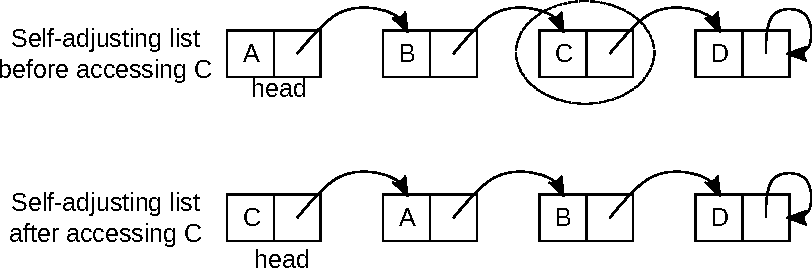
\includegraphics[width=.85\linewidth]{fig/mtf.pdf}
  \caption{A self-adjusting list containing nodes A,B,C and D serves the request to C and moves C to the front of the list to speed up future accesses to C.}
  \label{fig:mtf-example}
\end{figure}

Classic applications of MTF lists are information retrieval systems, compression~\cite{BentleySTW86}, etc. In network applications, however, where static linked lists enjoy wide applicability, e.g., for rule matching in OpenFlow and P4 reference software switches, packet classification in the Linux OS network stack (\texttt{iptables}), etc., so far we haven't seen many uses of the self-adjusting version, i.e., MTF lists. We imagine potential applications in packet classification (see later in \S\ref{sec:packet-classifier}), flow table lookup, evaluating rules in an intrusion detection system, etc.; in general, all networking use cases are relevant where ``matching'' a request against a list item is costly and the items do not lend themselves readily to be arranged into a fast lookup structure (like a search tree).



\noindent%
\textbf{Search trees.}


\begin{figure}
 \centering
 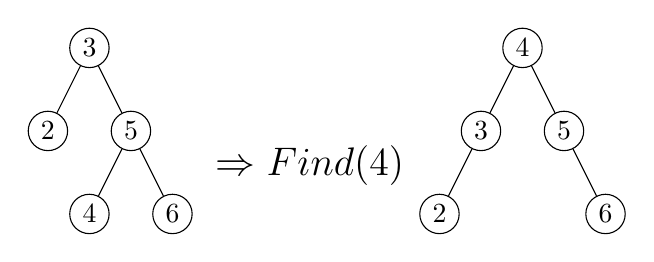
\begin{tikzpicture}[level distance=30pt,
   level 1/.style={sibling distance=30pt},
   level 2/.style={sibling distance=30pt},
   level 3/.style={sibling distance=30pt}]
   % Left
   \node[circle,draw,minimum size=0.5cm,inner sep=1pt] (3a) {3}
   child {node[circle,draw,minimum size=0.5cm,inner sep=1pt] (2a) {2}}
   child {node[circle,draw,minimum size=0.5cm,inner sep=1pt] (5a) {5}
     child {node[circle,draw,minimum size=0.5cm,inner sep=1pt] (4a) {4}}
     child {node[circle,draw,minimum size=0.5cm,inner sep=1pt] (6a) {6}}
   };
   % Right
   \node[circle,draw, minimum size=0.5cm, inner sep=1pt] (4b) at (5.5,0) {4}
   child {node[circle,draw,minimum size=0.5cm,inner sep=1pt] (3b) {3}
     child {node[circle,draw,minimum size=0.5cm,inner sep=1pt] (2b) {2}}
     child[missing] {}
   }
   child {node[circle,draw,minimum size=0.5cm,inner sep=1pt] (5b) {5}
     child[missing] {}
     child {node[circle,draw,minimum size=0.5cm,inner sep=1pt] (6b) {6}}
   };
   % Arrow
   \node (draw=none) at (2.8,-1.5) [font=\Large]{$\Rightarrow{Find(4)}$};
 \end{tikzpicture}
 \caption{Splay-tree with elements 2, 3, 4, 5, 6. After accessing node 4 it is moved to the root to speed up future accesses to it, while the search tree is kept almost perfectly balanced.}
 \label{fig:bst_root_3}
\end{figure}




\subsection{Locality-boosting load balancing}
\label{sec:lb-lb}

We call a request dispatching strategy that improves the temporal and\slash or spatial locality as experienced by the worker threads as a \emph{locality boosting load balancing policy}, and we identify such locality boosting load balancers as the first key ingredient in the superlinear scaling of distributed systems.

\begin{figure}
  \centering
  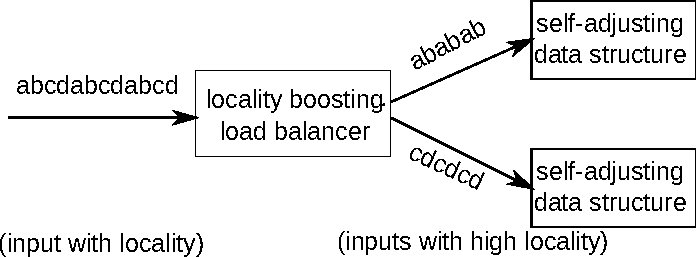
\includegraphics[width=.85\linewidth]{fig/schema.pdf}
  \caption{A locality boosting load balancer partitions the input sequence of a given locality into
    subsequences with higher locality. Self-adjusting data structures perform better on inputs with
    higher locality.}
  \label{fig:locality-boosting-lb}
\end{figure}

\subsection{Superlinear scaling}
\label{sec:arch-scaling}

% <PLACEHOLDER FOR MACIEK: discuss MTF lists without going into details, give examples with figs, and applications. Remember, we want to popularize the idea across the systems community, so be as gentle to practitioners as possible.>

show superlinear scaling with MTF

Indeed, a quick analysis proves that our MTF lists initially exhibit quadratic scaling over uniformly distributed requests. For a static linked list the worst-case lookup time is equals the length of the list, $m$, while for MTF it is rather the working set size $w\le m$ that determines lookup performance. This is because in MTF lists the working set will occupy the first $w$ positions in the list, which can be traversed in $w$ steps at most, and the inactive items will be moved to the back. Then, assuming that a hash-based load balancer partitions the $m$ possible requests over $k$ threads, each perceiving a working set size of $w=\frac{m}{k}$, the parallel MTF list will finish a lookup in amortized $\frac{m}{k}$ time. Plugging into Amdahl's law yields:
\begin{equation}\label{eq:mtf-perf}
  S_l(k) = \frac{T_l(1)}{T_l(k)} = \frac1{s + \frac{1-s}{k^2}} \enspace .
\end{equation}

For small values of $k$ we indeed obtain $O(k^2)$ scaling, despite that uniform request distribution is the worst case for self-adjustments. The fact that we see such speedups, even over a worst case input, hints at a great future potential over networking workloads that typically exhibit highly skewed request distributions~\cite{832484}.



\subsection{Simulations}
\label{sec:sims}


\begin{figure*}
  \begin{tabularx}{\textwidth}{D *{2}{s}}
    \multirow{-14.8}{*}{\subcaptionbox{List lookup/uniform input\label{fig:multicore-list-uniform-50k}}{\begin{small}
  \begin{tikzpicture}
    \begin{axis}[
      width=165pt,
      height=322pt,
      xlabel={number of CPU cores},
      x label style={at={(0.5,0.01)}},      
      ylabel={Speedup},
      y label style={at={(0.05,0.5)}},      
      xmin=1,
      xmax=48,
      xtick={1,12,24,36,48},
      ymin=0,
      ymax=3300,
      legend style = {
        anchor = north west,
        at = {(0.01, 1.01)},
        font=\tiny,
        % draw = none,
      },
      % scaled y ticks=false
      % no markers
      ]
      % use TeX as calculator:
      \addplot[black,mark=*] table[x=thread,y=speedup,] {fig/list/uniform-100k/multicore_mtf_modulo_uniform.txt};
      % \addlegendentry{Move-to-front/Local LB}
      \addplot[black,mark=+] table[x=thread,y=speedup,each nth point={3}] {fig/list/uniform-100k/multicore_linkedlist_modulo_uniform.txt};
      % \addlegendentry{Linked-list/Local LB}
      \addplot[black,mark=o] table[x=thread,y=speedup,each nth point={3}] {fig/list/uniform-100k/multicore_mtf_roundrobin_uniform.txt};
      % \addlegendentry{Move-to-front/Non-local LB}
      \addplot[black,mark=square] table[x=thread,y=speedup,each nth point={3}] {fig/list/uniform-100k/multicore_linkedlist_roundrobin_uniform.txt};
      % \addlegendentry{Linked-list/Non-local LB}
    \end{axis}
  \end{tikzpicture}
\end{small}

%%% Local Variables:
%%% mode: latex
%%% TeX-master: "../../../distributed_mrf"
%%% End:
}}
    & \subcaptionbox{Cache lookup/uniform input\label{fig:5}}{\pgfplotsset{
  RatePlot/.style = {
    tick pos = left,
    xtick align=outside,
    ytick align=outside,
    xlabel near ticks,
    ylabel near ticks,
    width=.4\textwidth,
    height=.3\textwidth,
    legend pos = north west,
    legend cell align=left,
    ylabel = {Throughput [Mpps]},
    xlabel = {number of CPU cores},
    xmin=1, xmax=32,
    ymin=0,
  },
  SpeedupPlot/.style = {
    RatePlot,
    ylabel={Speedup},
  },
  ClassBenchGroupPlot/.style = {
    group/group size = 1 by 2,
    group/horizontal sep = 0pt,
    group/vertical sep = 28pt,
  },
  ClassBenchRatePlot/.style = {
    RatePlot
  },
  ClassBenchSpeedupPlot/.style = {
    SpeedupPlot,
  }
}

%%% Local Variables:
%%% mode: latex
%%% TeX-master: "../distributed_mrf.tex"
%%% End:

%
\begin{small}
  % \tikzmath
  % {
  %   function est(\x)
  %   {
  %     if (\x < 10) then
  %     {
  %       return 0.1+0.9*(0.1*\x +(1-0.1*\x)*10)/\x;
  %     } else {
  %       return 0.1 + 0.9//\x;
  %     };
  %   };
  %   \a = est(4);
  %   \b = est(14);
  % }
  \begin{tikzpicture}
    \begin{axis}[
      width=165pt,
      height=120pt,
      xlabel={\#CPU cores},
      x label style={at={(0.5,0.04)}},
      ylabel={Speedup},
      % xlabel near ticks,
      % ylabel near ticks,
      y label style={at={(0.1,0.5)}},
      xmin=1,
      xmax=35,
      ymin=0,
      xtick={1,10,20, 30},
      % ymax=10,
      legend style = {
        anchor = north west,
        at = {(0.01, 1.01)},
        font=\scriptsize,
        % draw = none,
      },
      % no markers
      ]
      \addplot[SelfAdjustingSimMark,mark size=2pt] table[x=thread,y=speedup,each nth point={3}]{fig/cache/uniform-50k-2/mcore_cache_modulo_uniform.txt};
      % \addlegendentry{Local LB}
      \addplot[SelfAdjustingSimMark,mark=pentagon*,mark size=3pt,each nth point={3}] table[x=thread,y=speedup,each nth point={2}]{fig/cache/uniform-50k-2/mcore_cache_roundrobin_uniform.txt};
      % \addlegendentry{Non-local LB}
      % \addplot[domain=1:25,black,dashed]{x};
      % \addlegendentry{Linear scaling}
      % \addplot[domain=1:25,black,densely dotted]{1/(0.03+0.97/x)};
      % \addlegendentry{Amdahl's law}
      % \addplot[domain=0:25,black,densely dotted]{est(1.0)/est(x)};
      % \node at (100,100) {\a\b};
      % \addlegendentry{T}
      % \addplot[black,mark=o] table[x=thread,y=rate] {fig/cache/uniform-50k/multicore_cache_roundrobin_uniform.txt};
      % \addlegendentry{Round robin lb}
      % \addplot[black,mark=square] table[x=thread,y=rate] {fig/cache/uniform-50k/multicore_scache_roundrobin_uniform.txt};
      % \addlegendentry{staticcache / roundrobin}
    \end{axis}
  \end{tikzpicture}
\end{small}

%%% Local Variables:
%%% mode: latex
%%% TeX-master: "../../../distributed_mrf"
%%% End:
}\vspace{8pt}
    & \subcaptionbox{Tree lookup/uniform input\label{fig:2}}{\pgfplotsset{
  RatePlot/.style = {
    tick pos = left,
    xtick align=outside,
    ytick align=outside,
    xlabel near ticks,
    ylabel near ticks,
    width=.4\textwidth,
    height=.3\textwidth,
    legend pos = north west,
    legend cell align=left,
    ylabel = {Throughput [Mpps]},
    xlabel = {number of CPU cores},
    xmin=1, xmax=32,
    ymin=0,
  },
  SpeedupPlot/.style = {
    RatePlot,
    ylabel={Speedup},
  },
  ClassBenchGroupPlot/.style = {
    group/group size = 1 by 2,
    group/horizontal sep = 0pt,
    group/vertical sep = 28pt,
  },
  ClassBenchRatePlot/.style = {
    RatePlot
  },
  ClassBenchSpeedupPlot/.style = {
    SpeedupPlot,
  }
}

%%% Local Variables:
%%% mode: latex
%%% TeX-master: "../distributed_mrf.tex"
%%% End:

%
\begin{small}
  \begin{tikzpicture}
    \begin{axis}[
      width=165pt,
      height=120pt,
      xlabel={\#CPU cores},
      x label style={at={(0.5,0.04)}},
      ylabel={Speedup},
      y label style={at={(0.1,0.5)}},
      xmin=1,
      xmax=36,
      xtick={1,10,20,30},
      ymin=0,
      % ymax=370,
      grid=major,
      tick pos = left,
      legend style = {
        anchor = north west,
        at = {(0.01, 1.01)},
        font=\scriptsize,
        % draw = none,
      },
      % scaled y ticks=false
      % no markers
      ]
      % use TeX as calculator:
      \addplot[SelfAdjustingSimMark,mark size=2pt] table[x=thread,y=speedup,each nth point={3}] {fig/tree/uniform-500/multicore_wsplay_modulo_uniform.txt};
      % \addlegendentry{Splay-tree/Local LB}
      \addplot[StaticSimMark,mark size=3pt] table[x=thread,y=speedup,each nth point={3}] {fig/tree/uniform-500/multicore_wbtree_modulo_uniform.txt};
      % \addlegendentry{B-tree/Local LB}
      \addplot[SelfAdjustingSimMark,mark=pentagon*,mark size=3pt] table[x=thread,y=speedup,each nth point={3}] {fig/tree/uniform-500/multicore_wsplay_roundrobin_uniform.txt};
      % \addlegendentry{Splay-tree/Non-local LB}
      \addplot[StaticSimMark,mark=square,mark size=3pt] table[x=thread,y=speedup,each nth point={3}] {fig/tree/uniform-500/multicore_wbtree_roundrobin_uniform.txt};
      % \addlegendentry{B-tree/Non-local LB}
    \end{axis}
  \end{tikzpicture}
\end{small}

%%% Local Variables:
%%% mode: latex
%%% TeX-master: "../../../distributed_mrf"
%%% End:
}\vspace{8pt}
    \\
    & \subcaptionbox{List lookup/Zipf input\label{fig:3}}{\begin{small}
  \begin{tikzpicture}
    \begin{axis}[
      width=165pt,
      height=322pt,
      xlabel={number of CPU cores},
      x label style={at={(0.5,0.01)}},      
      ylabel={Speedup},
      y label style={at={(0.05,0.5)}},      
      xmin=1,
      xmax=48,
      xtick={1,12,24,36,48},
      ymin=0,
      ymax=3300,
      legend style = {
        anchor = north west,
        at = {(0.01, 1.01)},
        font=\tiny,
        % draw = none,
      },
      % scaled y ticks=false
      % no markers
      ]
      % use TeX as calculator:
      \addplot[black,mark=*] table[x=thread,y=speedup,] {fig/list/uniform-100k/multicore_mtf_modulo_uniform.txt};
      % \addlegendentry{Move-to-front/Local LB}
      \addplot[black,mark=+] table[x=thread,y=speedup,each nth point={3}] {fig/list/uniform-100k/multicore_linkedlist_modulo_uniform.txt};
      % \addlegendentry{Linked-list/Local LB}
      \addplot[black,mark=o] table[x=thread,y=speedup,each nth point={3}] {fig/list/uniform-100k/multicore_mtf_roundrobin_uniform.txt};
      % \addlegendentry{Move-to-front/Non-local LB}
      \addplot[black,mark=square] table[x=thread,y=speedup,each nth point={3}] {fig/list/uniform-100k/multicore_linkedlist_roundrobin_uniform.txt};
      % \addlegendentry{Linked-list/Non-local LB}
    \end{axis}
  \end{tikzpicture}
\end{small}

%%% Local Variables:
%%% mode: latex
%%% TeX-master: "../../../distributed_mrf"
%%% End:
}
    & \subcaptionbox{List lookup/uniform/single-core\label{fig:6}}{\begin{small}
  \begin{tikzpicture}
    \begin{axis}[
      width=250pt,
      height=170pt,
      xlabel={\#thread},
      ylabel={Goodput [million req/sec]},
      xlabel near ticks,
      ylabel near ticks,
      xmin=1,
      xmax=26,
      ymin=0,
      % ymax=10,
      legend style = {
        anchor = north west,
        at = {(0.01, 1.01)},
        font=\scriptsize,
        % draw = none,
      },
      % no markers
      ]
      \addplot[black,mark=*] table[
      x=thread,
      y expr=\thisrowno{4}/1000000
      ]{fig/list/uniform-10/singlecore_mtf_modulo_uniform.txt};
      \addlegendentry{MTF w/ hash-based lb}
      \addplot[black,mark=+] table[
      x=thread,
      y expr=\thisrowno{4}/1000000
      ]{fig/list/uniform-10/singlecore_linkedlist_modulo_uniform.txt};
      \addlegendentry{Static list w/ hash-based lb}
      \addplot[black,mark=o] table[
      x=thread,
      y expr=\thisrowno{4}/1000000
      ]{fig/list/uniform-10/singlecore_mtf_roundrobin_uniform.txt};
      \addlegendentry{MTF w/ round robin lb}
      \addplot[black,mark=square] table[
      x=thread,
      y expr=\thisrowno{4}/1000000
      ]{fig/list/uniform-10/singlecore_linkedlist_roundrobin_uniform.txt};
      \addlegendentry{Static list w/ round robin lb}
    \end{axis}
  \end{tikzpicture}
\end{small}

%%% Local Variables:
%%% mode: latex
%%% TeX-master: "../../../hotnets22"
%%% End:
}
  \end{tabularx}
  \caption{A figure}
  \label{fig:fig1}
\end{figure*}


Again, Amdahl's law perfectly describes the $3$ systems where at least one of the two components, locality-boosting load balancing and self-adjusting data structures, is missing. But when both ingredients are present we again identify a superlinear scaling profile, but this time in a much more pronounced form: with MTF lists and hash-based load balancing we see $150\times$ speedup with 24 cores compared to the single-threaded case. This is $6\times$ faster than what is predicted by Amdahl's law.

The results also corroborate that self-adjustments do have their cost: in Fig.~\ref{fig:multicore-list} we see that MTF lists, when used with non-locality-boosting load balancing (i.e., round robin), are slower than the non-self-adjusting versions.  This effect, however, is due to that the input is chosen to be the worst-case for MTF: for a skewed input distribution MTF shows visible performance margin over the static lists (see Fig.~\ref{fig:multicore-list-poisson}).

Finally, a surprising finding: Fig.~\ref{fig:singlecore-list-uniform-10} and Fig.~\ref{fig:singlecore-list-poisson-300} indicate that parallelization benefits performance even when we do not actually add more CPU power to the system! With uniformly distributed requests, for instance, we achieve $25\times$ speedup by spawning 25 parallel goroutines, while the total available CPU share is kept at $110$\%. % (i.e., $1,100$ milicores). % : roughly 100 mcores is kept for the load-balancer and the equivalent of 1 CPU core is available for the MTF threads.
And this is despite that the overhead of request generation, goroutine scheduling, and memory management all count towards the total system load and take away precious CPU time from the workload.


% LET's SKIP THIS: highly speculative!!!!!!!!!!!1
%
% \subsection{Revised Amdah's law}
% \label{sec:sims}

% An interpretation of superlinear scaling: if we introduce the notion of the ``virtual job size''. Implicit in Amdahl's law \eqref{eq:amdahl} is that the job size remains the same independently of $k$. Parallel self-adjustments, however, may actually \emph{decrease} the amount of work each worker has to perform per each request. Let $b(k)$ denote the ``virtual job size'' perceived by each worker when the number of  workers is $k$. We observe that in parallel self-adjusting systems $b(k)$ is decreasing in $k$; e.g., for MTF we have $b(k) = \frac1{k}$.

% the ``fixed size'' vs. ``scaled size'' distinction here: \emph{Fixed Time, Tiered Memory, and Superlinear Speedup}



% \begin{equation}\label{eq:revised-amdahl}
% S(k) = \frac{T(1)}{T(k)} = \frac{1}{s + \frac{1-s}{k^{\alpha}}} \enspace .
% \end{equation}

% Amdah's law for $\alpha=1$, distributed MTF scaling for $\alpha=1$, superlinear scaling with $\alpha>1$

%%% Local Variables:
%%% mode: latex
%%% TeX-master: "distributed_mrf"
%%% End:

